\section{El tablero y las leyes sobre historias}\label{leyes}
\begin{definicion}[Tablero residual]
Numeramos filas y columnas desde uno, con filas de arriba abajo y columnas de izquierda a
derecha. La casilla $(i,j)$ pertenece a $R_i,C_j,D_{i-j},A_{i+j-1}$. En las coordenadas
de~\cite{perfil,ultimas}, esta casilla es $(i-1,j-1)$, con la misma diferencia y con suma
$i+j-2$. Una diagonal, de cualquiera de las dos familias, está \emph{libre} cuando no contiene una
reina. Una línea está \emph{disponible} si es una fila o una columna vacía o una diagonal libre. El
tablero residual $B$ de una colocación parcial conserva las coordenadas originales y las $k$ filas y
$k$ columnas vacías. Sus \emph{cruces vacíos}, como en~\cite{ultimas}, son las $k^2$ casillas en que se
cortan una fila vacía y una columna vacía. Su soporte $E(B)$ consiste en los cruces vacíos cuyas dos
diagonales están libres, que son las \emph{casillas disponibles}.
\end{definicion}
Denotamos por $Q(B)$ el número de soluciones que prolongan la colocación de $B$, y por
$B+e$ el residual que resulta de insertar una reina en $e$. Llamamos \emph{hijo} de $B$ a cada $B+e$
con $e\in E(B)$, y \emph{padre} de esos hijos a $B$. El \emph{tablero inicial} $B_0$ es el residual
de la colocación vacía, de modo que $Q(B_0)=Q(n)$. Fijada una fila vacía $i$, toda completación
elige exactamente una de sus casillas disponibles, luego
\begin{equation}\label{particion}
 Q(B)=\sum_{e\in R_i\cap E(B)}Q(B+e).
\end{equation}
El residual sin filas vacías tiene una completación. Un hijo con una casilla recién ocupada
puede tener cero completaciones. La Figura~\ref{fig:historia} da un ejemplo de la partición.
\begin{figure}[htbp]
\centering
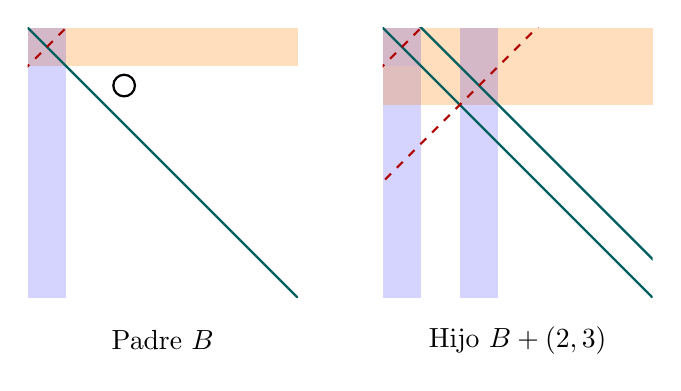
\begin{tikzpicture}[x=.49cm,y=.49cm]
 \foreach \etapa/\dx in {1/0,2/9.2}{
  \begin{scope}[shift={(\dx,0)}]
   \bcuadricula{7}
   \fill[orange,opacity=.26] (0,6) rectangle (7,7);
   \fill[blue,opacity=.17] (0,0) rectangle (1,7);
   \ifnum\etapa=2
    \fill[orange,opacity=.26] (0,5) rectangle (7,6);
    \fill[blue,opacity=.17] (2,0) rectangle (3,7);
   \fi
   \begin{scope}
    \clip (0,0) rectangle (7,7);
    \draw[teal!75!black,line width=.8pt] (.5,6.5) ++(-7,7) -- ++(14,-14);
    \draw[red!70!black,dashed,line width=.8pt] (.5,6.5) ++(-7,-7) -- ++(14,14);
    \ifnum\etapa=2
     \draw[teal!75!black,line width=.8pt] (2.5,5.5) ++(-7,7) -- ++(14,-14);
     \draw[red!70!black,dashed,line width=.8pt] (2.5,5.5) ++(-7,-7) -- ++(14,14);
    \fi
   \end{scope}
   \foreach \rr in {1,...,7}{
    \foreach \cc in {1,...,7}{
     \pgfmathtruncatemacro{\libre}{(\rr!=1)&&(\cc!=1)&&(abs(\rr-1)!=abs(\cc-1))}
     \ifnum\etapa=2
      \pgfmathtruncatemacro{\libre}{\libre&&(\rr!=2)&&(\cc!=3)&&(abs(\rr-2)!=abs(\cc-3))}
     \fi
     \ifnum\libre=1 \bmarca{7}{\rr}{\cc}\fi
    }
   }
   \breina{7}{1}{1}
   \ifnum\etapa=1
    \draw[black,line width=.8pt] (2.5,5.5) circle[radius=.28];
    \node at (3.5,-1.1) {Padre $B$};
   \else
    \breina{7}{2}{3}
    \node at (3.5,-1.1) {Hijo $B+(2,3)$};
   \fi
  \end{scope}
 }
\end{tikzpicture}
\caption{Una transición de un padre a un hijo en un tablero de orden siete. El padre tiene una reina
en la fila 1 y el hijo se obtiene al revelar la fila 2.
Las filas se numeran desde uno de arriba abajo y las columnas desde uno de izquierda a derecha.
Las coronas representan las reinas colocadas. Las bandas horizontales y verticales señalan sus filas y
columnas ocupadas. Las líneas continuas y discontinuas trazan las dos familias diagonales atacadas.
Cada punto indica una casilla disponible. En la fila siguiente, la $2$, las columnas $3,4,5,6,7$
tienen respectivamente $1,1,1,1,0$ completaciones, de modo que $Q(B)=4$. El círculo señala la elección
$(2,3)$ que produce el hijo de la derecha.}\label{fig:historia}
\end{figure}


\paragraph{Perfil y normalización.}
El Teorema~1.1 de~\cite{perfil} da el único perfil óptimo de masa uno, $\nu_1$, en el
cuadrado unidad. Denotamos su entropía por $s_1$ y escribimos $\Phi=s_1+1$. Como
en~\cite{perfil,ultimas,pred}, $m_D$ y $m_A$ son las proyecciones de $\nu_1$ sobre las dos familias
diagonales y $u_D=1-m_D$, $u_A=1-m_A$ sus vacancias. Si $f$ es una línea diagonal, $m_f$ y $u_f$
denotan los valores en $f$ de las funciones de su familia. Los Teoremas~1.2 y~1.3 y la Proposición~5.2
de~\cite{perfil} identifican los factores positivos y el límite en masa uno. El Teorema~7.7 del mismo
trabajo da el control hasta el extremo. Usamos la forma de~\cite[Sección~2]{pred},
\[
 \nu_1(r,c)=b_0 r_R(r)r_C(c)u_D(r-c)u_A(r+c),\qquad
 c_\nu\le\nu_1\le C_\nu,\quad \kappa_\nu\le u_D,u_A\le1.
\]
Las marginales de filas y columnas de $\nu_1$ valen uno, los factores son Lipschitz y $L_\nu$ denota
una constante de Lipschitz de $\nu_1$, como en~\cite{pred}. Las coordenadas continuas de la casilla
$(i,j)$ se toman en el centro de su celda de lado $1/n$.

\paragraph{Punto de Bethe y predictor.}
Escribimos RC por «filas y columnas». Como en~\cite{pred}, el \emph{punto de Bethe} de un residual
$B$ es el vector $p=(p_e)$, con un peso por casilla de $E(B)$, en el que se evalúa su predictor. Es
el punto estacionario de la entropía de Bethe
\begin{equation}\label{bethe}
 H_B(p)=-\sum_e p_e\log p_e+3\sum_e(1-p_e)\log(1-p_e)-\sum_fh_f\log h_f
\end{equation}
en el dominio $0<p_e<1/4$, $h_f>0$, con masas de fila y de columna iguales a uno. Aquí la
\emph{masa} de una diagonal $f$ es $\ell_f=\sum_{e\in f}p_e$ y su \emph{vacancia} es $h_f=1-\ell_f$.
La disponibilidad física es un indicador distinto de esta vacancia. En ese dominio $-H_B$ es
estrictamente convexa, de modo que hay a lo sumo un punto estacionario. Sólo usamos el punto de Bethe
en los tableros regulares de la Definición~\ref{def:regular} y en sus hijos, donde existe.

Cuando el grafo de filas y columnas del soporte es conexo, si $S_B$ es el operador de líneas, cuya
fórmula se da en la Sección~\ref{costes:normalizador}, y $\pdet$ es el producto de los autovalores
distintos de cero, el predictor satisface
\[
 L(B)=H_B(p)-\tfrac12\sum_e[\log(1-4p_e)-4\log(1-p_e)]
             -\tfrac12\log\pdet S_B+\tfrac12\log(4\pi k).
\]
El modo cero de $S_B$ es proporcional a $(\mathbf1_R,-\mathbf1_C,0)$; es el gauge de~\cite{pred}.
El cofactor de $S_B$ que se obtiene al suprimir la fila y la columna de una misma línea RC vale
$\pdet S_B/(2k)$, pues la componente correspondiente del vector unitario del modo cero tiene
cuadrado $1/(2k)$. Así, usar ese cofactor con $\tfrac12\log(2\pi)$, como
en~\cite[Secciones~6.1 y~7.1]{pred}, da el mismo $L(B)$.

El \emph{laplaciano de filas y columnas} de $p$ es, como en~\cite{pred}, el del grafo cuyos vértices
son las filas y las columnas vacías y en el que cada casilla disponible $e$ es una arista de peso
$p_e$ entre su fila y su columna. Su \emph{brecha} es su segundo autovalor más pequeño. Decimos que
$p$ cumple una \emph{cota de difusión} si $k\max_ep_e\le C$, una \emph{cota de vacancia} si
$h_f\ge\eta$ en toda diagonal y una \emph{cota de brecha} si esa brecha es al menos $\gamma$. Con
constantes $C,\eta,\gamma>0$ fijas, éstas son las cotas que piden los Teoremas~7.1 y~8.1
de~\cite{pred}: el primero para $k\ge\delta n$, y el segundo sin esa condición si la masa de cada
diagonal es a lo sumo un $\varepsilon$ pequeño.

Respecto de~\cite{pred} cambian algunas notaciones. Allí el hijo se escribe $B+c$, la fila se
sobreentiende en el cociente $\rho(B)$, que aquí es $\rho(B,i)$, y la masa y la vacancia de una
diagonal son $m_d$ y $h_d$; las demás diferencias se indican donde aparecen. Algunas letras, como $B$,
$E$, $J$, $S$, $T$ o $W$, designan en ciertas secciones objetos locales, que se definen donde aparecen;
por ejemplo, en la Sección~\ref{permanente} la letra $B$ denota la matriz $P-J_K$ y no un tablero.
Fuera del resumen y de la introducción, la letra $J$ no denota el operador de~\cite{pred}.

\paragraph{Leyes de revelado e inserción.}
Sorteamos uniformemente un orden $\sigma$ de las filas. Bajo la \emph{ley uniforme} $\mu$ elegimos,
de manera independiente de $\sigma$, una solución uniforme y revelamos sus reinas en ese orden.
Bajo la \emph{ley adaptativa} $\nu$, dada la siguiente fila $i$, elegimos $e$ con probabilidad
\[
 \nu_B(e\mid i)=\frac{\exp L(B+e)}{\sum_{e'\in R_i\cap E(B)}\exp L(B+e')},\qquad
 \rho(B,i)=\sum_{e'\in R_i\cap E(B)}\exp\{L(B+e')-L(B)\}.
\]
La \emph{ley auxiliar} $P^{\rm B}$ usa la misma fila uniforme y elige $e$ con probabilidad $p_e$. La
letra redonda de $P^{\rm B}$ y de su esperanza $\E_{\rm B}$ es de Bethe y no designa un tablero. Una
\emph{historia} es la sucesión de tableros $B_0,B_1,\dots$ que resulta, junto con el orden de las
filas. Decimos que un tablero con $k$ filas vacías tiene \emph{tamaño} $k$. En $B_t$ y en la historia
revelada $\mathcal F_t$, el índice $t$ cuenta inserciones. Al indexar por tamaño escribimos
$B^{(k)}=B_{n-k}$ y $\mathcal F^{(k)}=\mathcal F_{n-k}$. Esta última contiene las filas reveladas
hasta ese momento y sus casillas elegidas, antes de revelar la fila siguiente. En una historia
detenida, estos símbolos sólo se refieren a los niveles alcanzados.

\begin{definicion}[Tableros regulares y primera salida]\label{def:regular}
Fijamos $0<\delta<1$, $M=\lceil\delta n\rceil$ y un entero $K$ con $K_0\le K\le M$. El umbral $K_0$,
las constantes y las tolerancias que siguen se eligen en la Sección~\ref{meso:constantes}. Sea $B$ un
tablero de una historia, de tamaño $k$.
\begin{enumerate}[(a)]
\item \emph{Tramo macroscópico}, $k\ge M$. El tablero es \emph{regular} si la discrepancia $\Delta$
de la historia al llegar a él es menor que el radio $\varrho_{\rm mac}$ de la
Proposición~\ref{macro:parada}. La Sección~\ref{macro:observaciones} define esta discrepancia
con la partición $\mathcal I$, de paso $a_{\rm mac}$, de esa proposición.
\item \emph{Corte}, $k=M$. Se exige además que los observables de la
Sección~\ref{meso:regularidad} estén dentro de sus tolerancias de entrada y que
$D_{\max}(M)<\alpha M$, con la notación de la Sección~\ref{meso}.
\item \emph{Tramo mesoscópico}, $K\le k<M$. El tablero es regular si su punto de Bethe existe y
pertenece a la \emph{clase interior}: cumple las cotas de difusión, vacancia y brecha fijadas en la
Sección~\ref{meso:constantes} y la masa de cada diagonal es a lo sumo $\varepsilon$.
\end{enumerate}
La \emph{primera salida} de una historia es su primer tablero no regular, que llamamos \emph{tablero
de primera salida}. Su padre es regular. La historia se detiene en la primera salida o, si no la
hay, al llegar al tamaño $K$. El \emph{suceso de permanencia} $F$ consiste en que no haya salida:
todos los tableros hasta el de tamaño $K$, incluido éste, son regulares.
\end{definicion}
Para $n$ grande el tablero inicial es regular, pues su discrepancia es $O(1/n)$ (prueba de la
Proposición~\ref{macro:parada}). El punto de Bethe de un tablero regular cumple cotas de difusión,
vacancia y brecha con constantes fijas: en el tramo macroscópico por la Proposición~\ref{macro:maximo}
y el Corolario~\ref{macro:cambio}, y en el mesoscópico por definición. En el corte, las condiciones
adicionales lo sitúan ya en la clase interior, por la Proposición~\ref{meso:reconstruccion}. Sus
hijos, entre ellos el tablero de primera salida, heredan cotas del mismo tipo con constantes más
débiles, que llamamos \emph{cotas exteriores}; en el tramo mesoscópico, junto con una masa diagonal a
lo sumo $2\varepsilon$, definen la \emph{clase exterior}. En $\rho(B,i)$ intervienen todos los hijos
de $B$ en la fila $i$.

\begin{table}[htbp]\centering\small
\caption{Cómo se combinan las estimaciones en la comparación de los conteos.}
\begin{tabular}{@{}p{.31\linewidth}p{.59\linewidth}@{}}
\toprule Resultado & Estimaciones que utiliza \\ \midrule
Identidades \ref{hist:igualdad} y \ref{hist:inferior} & Partición por la siguiente fila y
normalización de las dos leyes.\\
Permanencia \ref{macro:cambio} & Balances \ref{macro:balances}, brecha \ref{macro:brecha},
reconstrucción \ref{macro:maximo} y parada \ref{macro:parada}.\\
Bandas \ref{prop:salida-banda-meso} & Prescripciones \eqref{prescr}, presupuesto
\ref{lema:presupuesto-meso}, concentración \ref{prop:concentracion-meso} y reconstrucción
\ref{meso:reconstruccion}.\\
Costes \ref{coste-macro} y \ref{coste-debil} & Comparación \ref{coste-comparacion} y, en el tramo
mesoscópico, normalizadores \ref{coste-normalizadores} y estimaciones del permanente
\ref{terminal-permanente} y \ref{terminal-normalizador}.\\
Último tablero \ref{terminal-error} & Geometría \ref{terminal-geometria}, pivotes
\ref{terminal-pivotes}, escalado \ref{terminal-escalado} y Proposición~3.1 de~\cite{dw}.\\
Teorema~\ref{princ} & Consistencia \ref{hist:consistencia}, cotas de salida y estimación
terminal bajo las dos leyes.\\ \bottomrule
\end{tabular}
\end{table}\begin{table}[!htbp]
\centering\small
\caption{Notación utilizada en la demostración.}
\label{tab:proof-notation}
\begin{tabular}{@{}p{.29\linewidth}>{\raggedright\arraybackslash}p{.65\linewidth}@{}}
\toprule
Símbolo & Significado \\
\midrule
$n,k$ & Orden del tablero inicial y número de filas vacías en el tablero residual. \\
$M,K$ & Corte $M=\lceil\delta n\rceil$ entre los dos tramos y tamaño terminal $K$. \\
$B_t,B^{(k)},B_\tau$ & Tablero tras $t$ inserciones, tablero con $k$ filas vacías
($B^{(k)}=B_{n-k}$) y tablero en la parada. \\
$\mathcal F_t,\mathcal F^{(k)}$ & Historia revelada, indexada por inserciones o por filas restantes,
con $\mathcal F^{(k)}=\mathcal F_{n-k}$. \\
\addlinespace[.22em]
$Q(B),L(B),g(B)$ & Conteo de completaciones, logaritmo del predictor y diferencia
$g(B)=\log Q(B)-L(B)$ cuando $Q(B)>0$. \\
$p_e,\ell_f,h_f$ & Peso de Bethe de la casilla $e$, masa de la diagonal $f$ y su vacancia
$h_f=1-\ell_f$. \\
\addlinespace[.22em]
$\mu,\nu,P^{\rm B}$ & Ley uniforme de revelado, ley adaptativa basada en el predictor
y ley auxiliar de Bethe. \\
$\tau,\rho(B,i),A_\tau$ & Tiempo de la primera salida o de la llegada al tamaño $K$, lo que ocurra
primero, cociente de normalización de la fila y logaritmo acumulado del cociente
$A_\tau=\sum_{t<\tau}\log\rho(B_t,i_t)$. \\
\addlinespace[.22em]
$F,G$ & Llegada al tamaño $K$ con regularidad hasta ese tablero inclusive, y subsuceso
$G=F\cap\{Q(B^{(K)})>0\}$. \\
$D_K$ & Suceso en el que dos cruces vacíos distintos en el tamaño $K$ comparten una diagonal. \\
\bottomrule
\end{tabular}
\end{table}

